

\tikzset{every picture/.style={line width=0.75pt}} %set default line width to 0.75pt

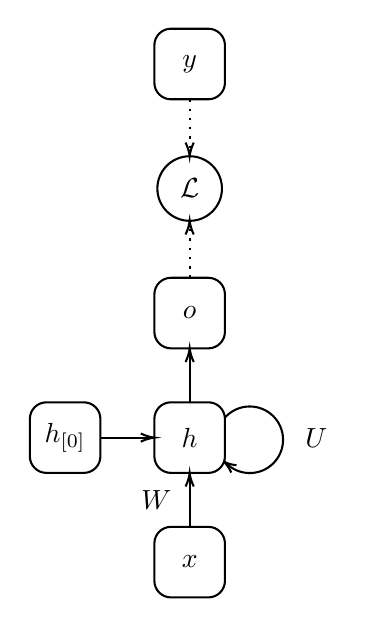
\begin{tikzpicture}[x=0.75pt,y=0.75pt,yscale=-1,xscale=1]
%uncomment if require: \path (0,300); %set diagram left start at 0, and has height of 300

%Shape: Circle [id:dp23367042930106008]
\draw   (107.92,216.04) .. controls (107.92,207.18) and (115.1,200) .. (123.96,200) .. controls (132.82,200) and (140,207.18) .. (140,216.04) .. controls (140,224.9) and (132.82,232.08) .. (123.96,232.08) .. controls (115.1,232.08) and (107.92,224.9) .. (107.92,216.04) -- cycle ;
\draw   (115.05,231.82) .. controls (114.1,229.66) and (112.86,227.9) .. (111.36,226.53) .. controls (113.14,227.51) and (115.22,228.09) .. (117.57,228.29) ;

% Text Node
\draw    (78,266) .. controls (78,261.58) and (81.58,258) .. (86,258) -- (104,258) .. controls (108.42,258) and (112,261.58) .. (112,266) -- (112,284) .. controls (112,288.42) and (108.42,292) .. (104,292) -- (86,292) .. controls (81.58,292) and (78,288.42) .. (78,284) -- cycle  ;
\draw (95,275) node   [align=left] {\begin{minipage}[lt]{20.400000000000002pt}\setlength\topsep{0pt}
\begin{center}
$\displaystyle \boldsymbol{x}$
\end{center}

\end{minipage}};
% Text Node
\draw  [fill={rgb, 255:red, 255; green, 255; blue, 255 }  ,fill opacity=1 ]  (78,206) .. controls (78,201.58) and (81.58,198) .. (86,198) -- (104,198) .. controls (108.42,198) and (112,201.58) .. (112,206) -- (112,224) .. controls (112,228.42) and (108.42,232) .. (104,232) -- (86,232) .. controls (81.58,232) and (78,228.42) .. (78,224) -- cycle  ;
\draw (95,215) node   [align=left] {\begin{minipage}[lt]{20.400000000000002pt}\setlength\topsep{0pt}
\begin{center}
$\displaystyle \boldsymbol{h}$
\end{center}

\end{minipage}};
% Text Node
\draw    (18,206) .. controls (18,201.58) and (21.58,198) .. (26,198) -- (44,198) .. controls (48.42,198) and (52,201.58) .. (52,206) -- (52,224) .. controls (52,228.42) and (48.42,232) .. (44,232) -- (26,232) .. controls (21.58,232) and (18,228.42) .. (18,224) -- cycle  ;
\draw (35,215) node   [align=left] {\begin{minipage}[lt]{20.400000000000002pt}\setlength\topsep{0pt}
\begin{center}
$\displaystyle \boldsymbol{h}_{[ 0]}$
\end{center}

\end{minipage}};
% Text Node
\draw    (78,146) .. controls (78,141.58) and (81.58,138) .. (86,138) -- (104,138) .. controls (108.42,138) and (112,141.58) .. (112,146) -- (112,164) .. controls (112,168.42) and (108.42,172) .. (104,172) -- (86,172) .. controls (81.58,172) and (78,168.42) .. (78,164) -- cycle  ;
\draw (95,155) node   [align=left] {\begin{minipage}[lt]{20.400000000000002pt}\setlength\topsep{0pt}
\begin{center}
$\displaystyle \boldsymbol{o}$
\end{center}

\end{minipage}};
% Text Node
\draw    (78,26) .. controls (78,21.58) and (81.58,18) .. (86,18) -- (104,18) .. controls (108.42,18) and (112,21.58) .. (112,26) -- (112,44) .. controls (112,48.42) and (108.42,52) .. (104,52) -- (86,52) .. controls (81.58,52) and (78,48.42) .. (78,44) -- cycle  ;
\draw (95,35) node   [align=left] {\begin{minipage}[lt]{20.400000000000002pt}\setlength\topsep{0pt}
\begin{center}
$\displaystyle \boldsymbol{y}$
\end{center}

\end{minipage}};
% Text Node
\draw (156,215) node   [align=left] {\begin{minipage}[lt]{20.400000000000002pt}\setlength\topsep{0pt}
\begin{center}
$\displaystyle \boldsymbol{U}$
\end{center}

\end{minipage}};
% Text Node
\draw (79,245) node   [align=left] {\begin{minipage}[lt]{20.400000000000002pt}\setlength\topsep{0pt}
\begin{center}
$\displaystyle \boldsymbol{W}$
\end{center}

\end{minipage}};
% Text Node
\draw    (95, 95) circle [x radius= 15.56, y radius= 15.56]   ;
\draw (95,95) node   [align=left] {\begin{minipage}[lt]{13.735995849609345pt}\setlength\topsep{0pt}
\begin{center}
$\displaystyle \mathcal{L}$
\end{center}

\end{minipage}};
% Connection
\draw    (95,258) -- (95,234) ;
\draw [shift={(95,232)}, rotate = 450] [color={rgb, 255:red, 0; green, 0; blue, 0 }  ][line width=0.75]    (6.56,-1.97) .. controls (4.17,-0.84) and (1.99,-0.18) .. (0,0) .. controls (1.99,0.18) and (4.17,0.84) .. (6.56,1.97)   ;
% Connection
\draw    (52,215) -- (76,215) ;
\draw [shift={(78,215)}, rotate = 180] [color={rgb, 255:red, 0; green, 0; blue, 0 }  ][line width=0.75]    (6.56,-1.97) .. controls (4.17,-0.84) and (1.99,-0.18) .. (0,0) .. controls (1.99,0.18) and (4.17,0.84) .. (6.56,1.97)   ;
% Connection
\draw    (95,198) -- (95,174) ;
\draw [shift={(95,172)}, rotate = 450] [color={rgb, 255:red, 0; green, 0; blue, 0 }  ][line width=0.75]    (6.56,-1.97) .. controls (4.17,-0.84) and (1.99,-0.18) .. (0,0) .. controls (1.99,0.18) and (4.17,0.84) .. (6.56,1.97)   ;
% Connection
\draw  [dash pattern={on 0.84pt off 2.51pt}]  (95,138) -- (95,112.56) ;
\draw [shift={(95,110.56)}, rotate = 450] [color={rgb, 255:red, 0; green, 0; blue, 0 }  ][line width=0.75]    (6.56,-1.97) .. controls (4.17,-0.84) and (1.99,-0.18) .. (0,0) .. controls (1.99,0.18) and (4.17,0.84) .. (6.56,1.97)   ;
% Connection
\draw  [dash pattern={on 0.84pt off 2.51pt}]  (95,52) -- (95,77.44) ;
\draw [shift={(95,79.44)}, rotate = 270] [color={rgb, 255:red, 0; green, 0; blue, 0 }  ][line width=0.75]    (6.56,-1.97) .. controls (4.17,-0.84) and (1.99,-0.18) .. (0,0) .. controls (1.99,0.18) and (4.17,0.84) .. (6.56,1.97)   ;

\end{tikzpicture}